\documentclass{article}
%\usepackage{includegraphicx}
\usepackage{sydewkrpt}
\usepackage{longtable}
\usepackage{array}
\usepackage{ragged2e}
\usepackage{amsmath}
\usepackage{amssymb}
\DeclareMathOperator*{\argmin}{\arg\!\min}
\DeclareMathOperator*{\argmax}{\arg\!\max}
\newcolumntype{P}[1]{>{\RaggedRight\hspace{0pt}}p{#1}}

%%%%%%%%%%%%%%%%%%%%%%%%%%%%
%%%    Begin Document    %%%
%%%%%%%%%%%%%%%%%%%%%%%%%%%%
\begin{document}
\pagenumbering{roman}

\waterlootitle{SYDE 461: Fall Term Final Report}{
  Group 2: Relay \\
  Adaptive Traffic Control Framework
}{
  Alex Huras -- 20344660\\
  D. Scott Neil -- 20349210\\
  Myles Tan -- 20349217\\
  Riley Donelson -- 20342815\\
  }

\dotableofcontents

\newpage
\doublespacing
\pagenumbering{arabic}
\section{Introduction}
\setlength{\parindent}{1cm}

This Design Project Implementation Plan will act as an update for interested parties on the progress made to date on Relay, the team's SYDE 461 Design Project. The problem background is discussed and a problem statement is provided. An overview of the solution is then presented: objectives, functional requirements, and design constraints are reviewed for each major solution component. An overview of the system design process is then presented, and a discussion on progress and insights to-date. Finally, an updated project plan and financial budget are presented.\\


\subsection{Background}
Motorists and pedestrians alike can relate to the frustration that comes from being stopped unnecessarily at a red light, waiting for it to turn green with no other cars in sight.
The intelligence of a traffic light can vary from a static, fixed timer, to a relatively intelligent node which considers existing traffic conditions, the performance of adjacent nodes, and the like.
However, even Adaptive Traffic Control (ATC) Systems today often irritate drivers as they are still unable to intelligently adapt to the wide variety of variables that affect traffic performance.\\

Large metropolitan areas are acknowledging the need for advanced traffic management systems as the size and density of urban areas continues to increase.
Over the past 29 years, the city of Los Angeles has developed a home-grown solution to handle the massive amounts of volume placed on their transportation networks, at an estimated cost of \$400 million to date \cite{la-atcs-article}.
The City of Montreal recently signed to adopt Transcore's TransSuite Advanced Traffic Management System (ATMS), which will control over 2000 intersections by completion \cite{montreal-transcore}.
There is strong need for ATCS technology in the world today, and there is a large opportunity for state-of-the-art ATC systems.\\

There are many industry-accepted and adopted ATC systems, such as LA ATCS, SCOOT, Trafficware, Spectrum by Miovision, InSync by Rhythm Engineering, Glide, ACS Lite by Centracs, and TransCore.
The method by which each system achieves enhanced performance varies: systems such as the LA ATCS implementation rely solely on road-planted magnetic sensors, whereas more advanced systems such as Miovision Spectrum utilize image processing technology.
The effectiveness of existing systems is noticeable but not impressive.
For example, LA ATCS, the largest ATCS implementation in North America, claims to reduce drive time on major corridors by 12\% \cite{la-atcs-article}, this aggregate statistic heavily biases freeway control but is currently suboptimal for average intersections.
Today's ATCS systems provide incremental gains on existing traffic control paradigms which have not changed for generations.\\

Significant advancements in Adaptive Traffic Control systems have been seen in academia.
Research efforts have been made towards novel architectures such as agent-based distributed systems which implement advanced machine learning and neural network concepts.
These revolutionary concepts have demonstrated significant gains in efficiency via simulated comparisons to existing industry systems \cite{1688100, 5073360, uot-article}, and some have even run trial implementations on real transit networks \cite{uot-article}.
However, these novel methods have yet to gain traction in industry, which continues to implement incremental advances based on old traffic control paradigms.\\

Furthermore, access to the data from such systems is largely kept for internal analysis by the government organizations, suffocating further technological development by industrial and academic organizations.
No existing systems offer consumer access to the system's data in any form.
It takes little imagination to realize the possible benefits, if real-time traffic network information was available to consumer route-planning technology.\\

In essence, there currently exists no industry-accepted Adaptive Traffic Control System, which adequately meets current and future transportation demands on urban road networks.
Current solutions offer incremental improvements on old strategies, and provide insufficient performance increases.
Without such a system, the inefficiency of crucial transportation methods will continue to increase, leading to greater financial, environmental, and sociological consequences.
A fundamentally different approach to traffic control is necessary, one which fully utilizes today's technological advances and novel methods for approaching complex, network-based problems.
The solution must meet the needs of transportation authorities, who will be responsible for overseeing the performance and maintenance of the system, and are ultimately responsible for the system.
The solution must also meet the needs of the population which it serves, providing transparent access to it's operation and allowing consumers to take full advantage of the information and insight which the system can provide.
The advantages of the system should be apparent and noticeable by both stakeholders, and finally, the system must be reliable and robust, due to the severe safety and efficiency consequences of failure and poor performance. The Relay system will be a proof of concept for \emph{democratic}, distributed intelligent traffic control systems.\\

\subsection{Proposed Solution}

Our solution: ``Relay'' is a distributed Adaptive Traffic Control System, that models each intersection in a city as an individual node in an online network.
Each node is capable of making real-time traffic decisions based on arbitrary data inputs.
These inputs may include knowledge of traffic at the intersection, historical trends of traffic data, traffic performance at adjacent nodes, and auxiliary data inputs such as weather conditions (and their expected effect on the network), and abnormal system behaviour.\\

On top of this system will sit an analysis and insight application known as the Relay Enhanced Interface, which will allow users to interact with the network.
An intuitive, information-rich interface will provide traffic authorities with necessary system information to monitor its performance, interact with the Relay Framework if necessary, and aid in auxiliary tasks.
This new interface will drastically decrease the cognitive workload of traffic authorities by providing an easy to understand information display, in contrast to existing ATCS interfaces which are overwhelming and poorly composed.\\

A different, publicly accessible interface will provide high-level performance information for the public to access, called the Relay Basic Interface.
This will fundamentally shift the way the public thinks about traffic, enabling the population to truly understand how the system works and how traffic decisions are being made, dramatically increasing the transparency of the network controller.
This has the opportunity to allow the public to make more intelligent route planning and transportation decisions on true traffic information, or even possibly democratizing signal control techniques.

\section{Design Objectives and Requirements}

This section outlines the high-level needs of the project, as well as detailed requirements, specifications, and constraints that the group will be facing throughout the next term.
Overall, the project will be successful if a system is created that (in simulation) improves the flow of traffic in a city.
It is required that the proposed system be inexpensive, highly robust, and arbitrarily scalable.
It must comply with all safety/legal regulations that are standard in a city, and should make minimal assumptions about the underlying signal timing infrastructure (i.e. not all intersections have advanced, accurate sensors).
At a lower level, a byproduct of a successful system will be reduced stop-time at an intersection under varying conditions.\\

\subsection{Relay Framework}

This section will focus on the two main back-end (non client facing) components of the system, the network of intersections and the algorithms that control them.
Below are the main objectives and requirements of these components.
These objectives attempt to address the problems with current traffic systems.\\

\subsubsection{Objectives and Requirements}

One of the main problems with current implementations and designs of some intelligent traffic systems is that they focus specifically on arterial corridors \cite{ACS:2008}.
While this dramatically simplifies the problem of agent-based control, it significantly reduces the possible benefits of the system.
This simplification is made because creating a large-scale distributed network of intersection agents is difficult and requires high coordination between units.
This is one of the focuses of our solution: create a network of nodes that can easily communicate and adapt to their surroundings, to allow us to implement a complex traffic network.
Testing will be performed on simpler models (small network size, limited input information) first to ensure the system is functioning properly, but ultimately we will execute simulations on a large network to evaluate this objective.
The network extent will be measure by the percentage of intersections in the network that are connected.\\

Next, the system should be able to change signal timings at non-fixed intervals (i.e. be acyclic), and do so \emph{online} (dynamically, adaptively).
What this means is that the system does not update the timings at a specific amount of time (e.g. 5 minutes), but rather continuously adjusts and adapts based on information collected in real-time.
If a large traffic system is expected at an intersection in the next minute, the actor of interest should be able to respond to this as soon as it becomes aware, and take the prediction into account when selecting timings.
While this problem is being addressed in research it is still not implemented in many commercial traffic systems \cite{155481, 5349439, ACS:2008}, and truly acyclic control is still in its infancy in industry.
Our solution will also address this issue, utilizing existing research findings where applicable.
This will be measured by the saturation of the intersection (i.e. the volume/flow-to-capacity ratio).
This tracks how much load the intersection is handling versus is potential capacity for each behaviour.\\

Thirdly, the benefits of these systems can sometimes be unclear.
While it is apparent that such a system should increase traffic flow through the network, more specific, low-level data is rarely provided.
As a research problem, modern traffic control systems measure their effectiveness in simulation against benchmark behaviours (such as fixed timings), and as such are very difficult to evaluate outside of their originating simulated context.
Specifics of this will be covered in the Interface section below, but the back-end must be constructed in such a way that this information can easily be queried and used, making all performance data transparent.
If the system is performing poorly, it should be obvious.
We will create an open platform with data streaming capabilities, so that the user-facing application gives greater insight into the current traffic conditions.

Lastly, while we will not be addressing this problem in the proposed solution, cost of implementation is a significant factor in traffic engineering \cite{ACS:2008, Miovision:2012}.
We are not considering cost of implementation in our design as we are more interested in and focused on conducting research/developing a proof of concept in the fields of traffic engineering, data visualization, and distributed computing.

Below, Table \ref{table:proj-reqs} outlines the objectives identified above, plus others that the group has specified.
These other objectives do not directly relate to the problems stated, but address items that are important in an adaptive system.
The last objective is something that we will attempt to incorporate, but is a secondary item and not of the highest-priority. \\

\begin{longtable}[htbp] {| P{4.5cm} | P{6cm} | P{4.5cm} |}
    \hline
    Objective                                                 & Requirement                                                                                        & Metric/Measurement  \\ \hline
    Applied to entire traffic network               & Most, if not all, intersections in the network are connected                 & Percentage of intersections controlled \\ \hline
    Acyclic light timing                                   & Timings update at non-fixed intervals; when data is received              & Arterial travel time, mean delay of vehicles \\ \hline
    Open and accessible data                       & Generated traffic data should be query-able and usable by front-end solution     & N/A       \\ \hline
    Reduced commute time, for average user      & Travel time down main roads in a city should be decreased from current conditions               & Arterial travel time,
mean delay of vehicles  \\ \hline
    Reduced stop frequency                          & Minimize variance of travel speed (smooth flow)                     & Variance of travel speed                                \\ \hline
    Reduced stoppage time                           & Minimize time spent waiting at intersection                          & Intersection delay, mean stoppage time of vehicles, queue length distributions \\ \hline
    System Resilience and Robustness                               & The system should respond well to external disturbances such as system failures, acts of god, etc. & Minimized degradation in existing system performance metrics                          \\ \hline
    Emergency/High Occupancy Vehicle Priority    & System should safely prioritize emergency vehicles along major routes    & Tentatively out of scope        \\ \hline
\caption{Project Requirements}
\label{table:proj-reqs}
\end{longtable}

\subsection{Relay Interface}
The second major component of our solution is a graphical user interface (GUI), for understanding and interacting with the Relay Framework.
As with the current state of the art, traffic engineers typically use a GUI which is connected to their ATCS to observe network and intersection performance.
Figure \ref{fig:scats-screenshot} shows an example of the GUI for monitoring an intersection in SCATS, an existing Adaptive Traffic Management System \cite{scats}.\\

\begin{figure}[htbp!]
  \begin{centering}
    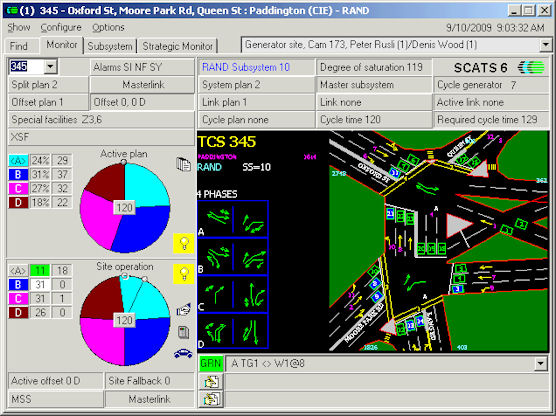
\includegraphics[scale=0.8]{figures/scat-screen.jpg}
    \caption{The SCATS interface is overwhelming and not optimized.}
    \label{fig:scats-screenshot}
  \end{centering}
\end{figure}

In general, traffic control systems are extremely data-intensive, and can place high information processing loads on the user.
It is important that GUIs are designed to minimize the cognitive processing required by the users, and provide intuitive and informative views on the network.\\

The SCATS interface shown in Figure \ref{fig:scats-screenshot} has many drawbacks in terms of it's efficiency in conveying information to the user.
Problems such as information redundancy, unclear interface functionality, poor hierarchy design, and poor data visualization methods are main contributors to this problem.
Most other existing ATCS GUIs have similar interface design paradigms, and thus face similar setbacks \cite{la-atcs-brochure}.\\

This motivates our first high-level objective for the Relay Interface component of the Relay solution, which is to create a GUI which is intuitive, informative, and clean, that traffic engineers and similarly informed users can utilize to monitor the ATCS.
This will be referred to as the Enhanced Interface.\\

Typically, external access to TCS information is restricted to contracting organizations working on the system, and sometimes for research initiatives.
Where allowed, public availability of traffic information is limited to annual reports of basic traffic flow metrics across the network.
There are considerable arguments which can be made for the disclosure of this data on a real-time basis for public consumption.
The most significant use case for public access to TCS data is for intelligent route planning.
Currently, route-planning services such as Google Maps rely on measurements taken by consumer GPS-enabled devices to determine traffic conditions and provide more intelligent route planning.
However, insights into traffic patterns derived from this method are extremely basic, as seen in Figure \ref{fig:apple-maps}.\\

\begin{figure}[htbp!]
  \begin{centering}
    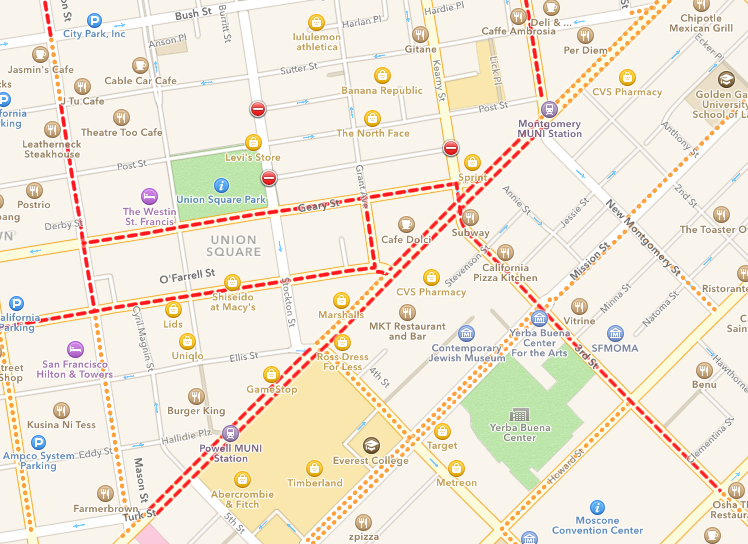
\includegraphics[scale=0.46]{figures/apple-maps.png}
    \caption{Basic traffic insight provided by Apple Maps.}
    \label{fig:apple-maps}
  \end{centering}
\end{figure}

A route-planning service which utilized ATCS data could provide unprecedented accuracy with respect to traffic congestion for route planning.
Route-planning could even be enhanced, using the ATCS traffic-timing information and predictive traffic models.
On a higher-level, providing public access to infrastructure enables more informed public opinions and objective insight into the governmental operations.
Such data could be used by the public to further public initiatives and conversations around public decisions and policies, as well as rebalancing load on the network by encouraging drivers to take less congested routes.
This type of transparency follows the modern trend in ``open data''.\\

The second objective of the Relay GUI is to encourage and provide public access to the ATCS information through a public, basic interface.
Within the scope of this project, the interface will support a consumer-facing interface to provide users with high-level understanding of traffic performance throughout the city.\\

Table \ref{table:interface-objectives} lists the objectives and functional requirements for the Relay Interface.
Each functional requirement is prepended with the objectives it applies to, and many of them belong to both objectives.
Measurements of success for each functional requirement are either binary or a 1 to 5 Likert Scale.
Binary assessment has been used to assess functional requirements where success is objective, such as the ability to zoom and pan a map.
Likert scale assessment has been used where the success of implementation is more subjective.
Success will be based on feedback to the assigned questions in user testing.
Seeing as the objective relate to different users, responses from the appropriate user group will be used to calculate the success measurement.
For example, a the success measurement of a functional requirement which relates only to traffic engineers and similar users will only consider responses from testers of that background. \\

\newpage
\begin{table}[htbp!]
\begin{centering}
\begin{tabular}{|c|p{8cm}|}
\hline
\textbf{Objective Number} & \textbf{Objective} \\ \hline
Objective 1 & Create a user interface for traffic engineers and similar users with sufficient knowledge in traffic engineering to monitor and interact with the Relay Framework. \\ \hline
Objective 2 & Create a user interface for the public which provides high-level performance and status information regarding the Relay Framework. \\ \hline
\end{tabular}
\caption{Numbered Objectives for reference in Table \ref{table:interface-functional-requirements}.}
\label{table:interface-objectives}
\end{centering}
\end{table}

\begin{longtable}[htbp!] {|p{6cm}|p{6cm}|}
\hline
\textbf{Functional Requirement} & \textbf{Measure} \\ \hline
(1) Traffic engineers and similar users must be able to access an authentication-restricted interface which allows them to monitor and interact with the Relay Framework, referred to as the enhanced interface. & Does the interface exist? (Y/N) Is access limited to specific users? (Y/N) \\ \hline
(2) Public users must be able to access a publicly available interface which allows them to monitor and learn the state of the network, referred to as the public interface. & Does the interface exist? (Y/N) Is it publicly accessible? (Y/N) \\ \hline
(1 \& 2) Both interfaces must provide a geographic, visual representation of the ATCS network (map). & Is there a visual representation of the network? (Y/N) \\ \hline
(1 \& 2) The map of the network must provide an overall understanding of the state/performance of the network. & 1 to 5 Likert scale agreement rating: The map provides me with a strong understanding of the overall state/performance of the network. \\ \hline
(1 \& 2) The user should be able to select from various data layers to be shown on the map. & Can the user select from multiple data layers to be shown on the map? (Y/N) \\ \hline
(1 \& 2) The user must be able to pan and zoom within the map to further explore the network. & Can the user manipulate the map? (Y/N) \\ \hline
(1 \& 2) The visual representation of the network must highlight abnormalities and problems within the network for the user. & 1 to 5 Likert scale agreement rating: From the map, I can immediately identify abnormalities/problems within the network? \\ \hline
(1 \& 2) Both interfaces must contain a dashboard for containing high-level information such as network metrics, alerts, and visualizations. & Is there a dashboard? (Y/N) \\ \hline
(1 \& 2) The dashboard must be toggle-able, such that the user can choose to hide or show it. & Can the user toggle the dashboard into and out of sight? (Y/N) \\ \hline
(1 \& 2) The dashboard must contain user-friendly, network-wide metrics relevant to the performance/state of the Relay Framework. & 1 to 5 Likert Scale agreement rating: The dashboard contains all the network-wide metrics needed to understand the state of the system. \\ \hline
(1) The dashboard on the enhanced interface must provide technical, network-wide metrics relevant to traffic flow. & 1 to 5 Likert scale agreement rating: The enhanced interface dashboard contains the required technical metrics for a traffic engineer or similar user to understand the state/performance of the network. \\ \hline
( 1 \& 2) The user must be able to see basic information about an intersection when clicking on one. & Does clicking on an intersection reveal basic information about the intersection? (Y/N) \\ \hline
(1) The user must be able to see more detailed information about the intersection. & Is the user able to see more detailed information regarding the intersection? (Y/N) \\ \hline
(1) The detailed view of a single intersection must provide more detailed information with regards to the intersection's state and performance, such as performance metrics and current signal timings. & 1 to 5 Likert scale agreement rating: The enhanced view of an intersection provides all the necessary metrics and visualizations to understand the state/performance of the intersection. \\ \hline
(1 \& 2) The user should be able to search for specific intersections within the Relay Framework. & Can the user search for specific intersections in the network? (Y/N) \\ \hline
\caption{Functional requirements for the Relay Interface.}
\label{table:interface-functional-requirements}
\end{longtable}

\subsection{Design Constraints}

There are multiple design and environmental constraints that will affect the final solution created.
The main items are: limited timeline, simulating traffic, and traffic regulations.\\

Firstly, with only approximately 6-months to reach a final implementation it will be very difficult to create a polished product.
Because adaptive traffic control is such a large problem, the team will only focus on specific aspects of it.
To help us tackle traffic control itself, we will assume that we have perfect traffic data and built a system on top of this.
While this will not change the final product, it eliminates some of the challenges with creating such a system.\\

Secondly, simulating a traffic system is difficult, and obtaining real traffic data is extremely difficult.
While there are tools available for this, we currently have not found one (that we have access to) that will work effectively.
The team will continue to investigate this, but may either have to revert to Vissim (provided by supervisor) or creating our own simulation.
If one of these actions is required, the final prototype will not be as feature-rich as desired.
Time would be directed towards one of these tasks, which would detract from progress on the actual solution.
Also, real traffic data would need to be provided by a municipality and it is very unlikely that they would be willing to provide this within such a constrained time period.
This option will not be pursued because of this difficulty and short timeline.\\

Next, regional traffic regulations and laws will affect how the system acts or is implemented.
Parameters within the system will need to be adjusted to account for these, and it should be easy to do so.
Adjustments could take the form of minimum/maximum signal time, allowable behaviours, arterial roads (not related to regulations, but would be custom to the system), and any other specific rules to a neighbourhood, city, road, or other road component.
Additionally, the behaviours must only represent the legal states for a given intersection.
Invalid light patterns (e.g. perpendicular green lights) need to be avoided and rules will be programmed into the system to accommodate this.\\

\subsection{Implications}

Adaptive Traffic Control Systems have many positive social and environmental implications as a byproduct of improving traffic flow through a city.
A few of these are decreased gas consumption, quicker travels, and reduced congestion.
It is important to note that these are not direct goals of the implementation, but rather beneficial external consequences of effective traffic control, that naturally extend from effectively adapting signal timings.
The proposed solution thus focuses on local intersection performance, and builds out from there.

An adaptive traffic system also has the ability to be modified for region and time specific parameters.
Unlike previously discussed, this would entail modifications for specific road conditions, neighbourhoods, and/or vehicle types.
Adapting for changing weather and road conditions improves the safety of travellers through the system by changing signal timings to reflect changing driving speeds.
For example, in icy conditions rather than improve intersection volume, it could hypothetically be more beneficial to reduce the amount of acceleration undergone by vehicles, resulting in a lower average speed, but safer transportation environment for all.
By optimizing for these new conditions it would attempt to ensure traffic is still flowing smoothly.
Incorporating more external data, such as school times, locations, and days, allows the system to dynamically control car flow through school zones.
This would help to increase safety in these areas by working to either route cars away from these zones, or adapting to reflect slower speed limits during ``school hours''.
Also, by weighting certain vehicles differently (e.g. giving priority to buses or other high occupancy vehicles), total person throughout can be increased.
This type of bias will be tested in the simulations, and could potentially increase the attractiveness of public transportation.

\newpage
\section{System Design}

This section contains high level design overviews of the various components of Relay, including specific technology/design selections and considerations.
Relay is broken up into relatively independent modules that are responsible for user interaction, application service, and intersection control and synchronisation.\\

\subsection{Front-End Design Approach}

For as long as cities have existed, traffic (and traffic-related byproducts such as pollution, accidents, and road-rage) has been a significant drawback to urban living.
Adaptive Traffic Control Systems have typically been too expensive for widespread implementation in all but the most horrifically congested urban areas \cite{la-atcs-article}.
As such, one of the main goals of the design is to demonstrate the utility of arbitrarily large distributed (rather than centralized) Adaptive Traffic Control Systems that change their behaviours in real time.
Additionally, as a potential public works project, sufficient emphasis must be placed on reliability, redundancy, and transparency.
From experience, we know that natural disasters and power outages can simultaneously take down multiple blocks of a city.
Our solution should be able to operate in highly volatile environments, with imperfect or otherwise untrustworthy information, and as a whole: attempt to fail gracefully - intelligently diverting traffic from fault zones.
This continuous process of adaptation and optimization shouldn't be hidden either.
Through the use of the Relay Interface, the models and data behind the intersection controllers should be exposed and understandable to users of the system.
This includes not just the standard groups of urban traffic engineers, but also inhabitants of the city.\\

The concept generation is delineated into several independent modules - each with their own implementation details, that as a whole, form Relay.
At a high level, the system can be broken into two independent modules: the Interface (including associated technologies and processes), and the Framework, which consists of everything required to operate intersection controllers (agents).\\

A highly iterative design process was employed for each component of the project, at each stage of prototype development.
The following outlines the specific design solution for the prototype, and validation for continued project development.\\

\subsubsection{Research and Concept Generation}

The prototype design began with intensive research into both the current state of the art in traffic control and intelligent traffic systems, as well as into visualization techniques for traffic data and the relevant metrics that accompany it.
Alongside this research, early-stage design ideas were developed in a fast-paced brainstorming environment, in order to generate as many concepts as possible.\\

Consisting mainly of low-fidelity sketches and whiteboard illustrations, many visualization strategies were brought up and analyzed based on how well they represent the data at hand, how easy it is to understand the visualization, aesthetic appeal, and technical feasibility.
An idea at this stage was to use histograms to visualize traffic data as real-time probabilities in motion along busy roads.
A second idea involved a more typical coloured dotted-line approach - as seen in popular applications such as Google Maps and Apple Maps.
A third idea existed as a heat map of overlaying translucent circles, whose presence indicate traffic density based on intensity of colour.
This stage of design was also important for scoping of the project, and gaining a full understanding of what a realistic prototype and final product will look like.
Technical implementations were discussed and explored for each concept, as well as auxiliary features and requirements that are incorporated into a useful web application.\\

\subsubsection{Wireframing}

The design process swiftly moved into a brief wireframing stage, to further validate generated concepts, and weigh their feasibility and effectiveness in implementation.
At this stage, the team also began to refine a visual aesthetic and style to define the look and feel - and more subtly - the tone of the product.
Figures \ref{fig:wire-1} - \ref{fig:wire-4} show sketches and wireframes of the early-stage visualization concepts for the interactive data-displaying application.\\

\begin{figure}[htbp!]
  \begin{centering}
    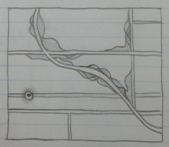
\includegraphics[scale=1]{figures/wire-1.png}
    \caption{Initial wireframe for histogram approach.}
    \label{fig:wire-1}
  \end{centering}
\end{figure}

\begin{figure}[htbp!]
  \begin{centering}
    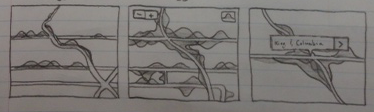
\includegraphics[scale=1]{figures/wire-2.png}
    \caption{Application wireframes showing interaction controls and pop-up menu.}
    \label{fig:wire-2}
  \end{centering}
\end{figure}

\begin{figure}[htbp!]
  \begin{centering}
    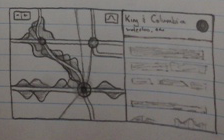
\includegraphics[scale=1]{figures/wire-4.png}
    \caption{Sketch of potential side menu for the Relay Interface application.}
    \label{fig:wire-3}
  \end{centering}
\end{figure}

\begin{figure}[htbp!]
  \begin{centering}
    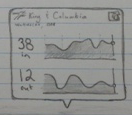
\includegraphics[scale=1]{figures/wire-5.png}
    \caption{Sketch of a detailed pop-up menu showing intersection data.}
    \label{fig:wire-4}
  \end{centering}
\end{figure}

As can be seen in Figures \ref{fig:wire-1} - \ref{fig:wire-4}, various overlay techniques using both histograms and circular polygons on a map of a city were explored here.
The histogram approach sought to model each vehicle (or small group of vehicles) on the road as a probability density function that could be moved along a road based on knowledge of traffic presence at each intersection, and speed limit data on each road.
More vehicles means more histograms, shown as translucent graphs which when overlayed, become more and more opaque, thus indicating a higher traffic density in that area.
Response for this concept was generally critical, as probability functions overlayed on a map are not particularly easy to understand, at least not immediately on first-glance.
It was evident at this stage that a simpler - more intuitive - visualization was needed for this application to be useful for both consumers and traffic engineers.\\

Through exploration of the circular polygon heat-map concept, a more agreeable solution was found.
This concept modelled traffic data on more of a per intersection basis.
In other words, when an intersection is experiencing a high volume of traffic, a translucent circular polygon is triggered and overlayed onto a map of the city at the longitude and latitude of the intersection.
The size of the circle is positively correlated to the volume of traffic at the intersection.
A second degree of data is then shown through use of colour, to illustrate the performance of the intersection itself.
In other words, how well the intersection is moving traffic given it's high-volume state.
It was agreed upon that a well-performing high-volume intersection should receive a colour that is neutral, while a high-volume intersection with poor performance should emit a colour that indicates that something is wrong, such as orange or red.\\

It can also be seen in the figures that other components of the prototype application were accounted for in the wireframes.
These include interactions such as pop-up dialogues, highlighting routes and communicating intersections, as well as a side-panel for showing detailed metrics on intersection and overall city-wide traffic performance.
From this stage, the prototype moved to a mid-fidelity phase to further build out the concepts and refine the aesthetic of the application.\\

\subsubsection{Mid-Fidelity Prototype}

At the mid-fidelity prototyping phase, the wireframes and sketches were taken into software such as Photoshop, Illustrator, Quartz Composer, and After Effects to create static and pseudo-working application mockups.
This stage also involved a great deal of consideration into the design of the map itself, in addition to the data.
This required a detailed look into cartographic design and styling techniques, based on the needs of our application.
Given that this application is solely for viewing traffic conditions and relevant data, an immediate requirement for the map was to be as minimal as possible.
Basic road labels on a dark palette were found to be some of the only necessary cartographic features in the design of the map, and as such the team was able to remove a great deal of unnecessary clutter such as restaurants, transit locations, schools, and other small urban landmarks.
The map was styled using a desktop application known as TileMill, as well as an open source web application called CloudMade.
The custom-made style package has been made freely available for the public on the CloudMade service, and can be seen below in Figure \ref{fig:map-styling}.\\

\begin{figure}[htbp!]
  \begin{centering}
    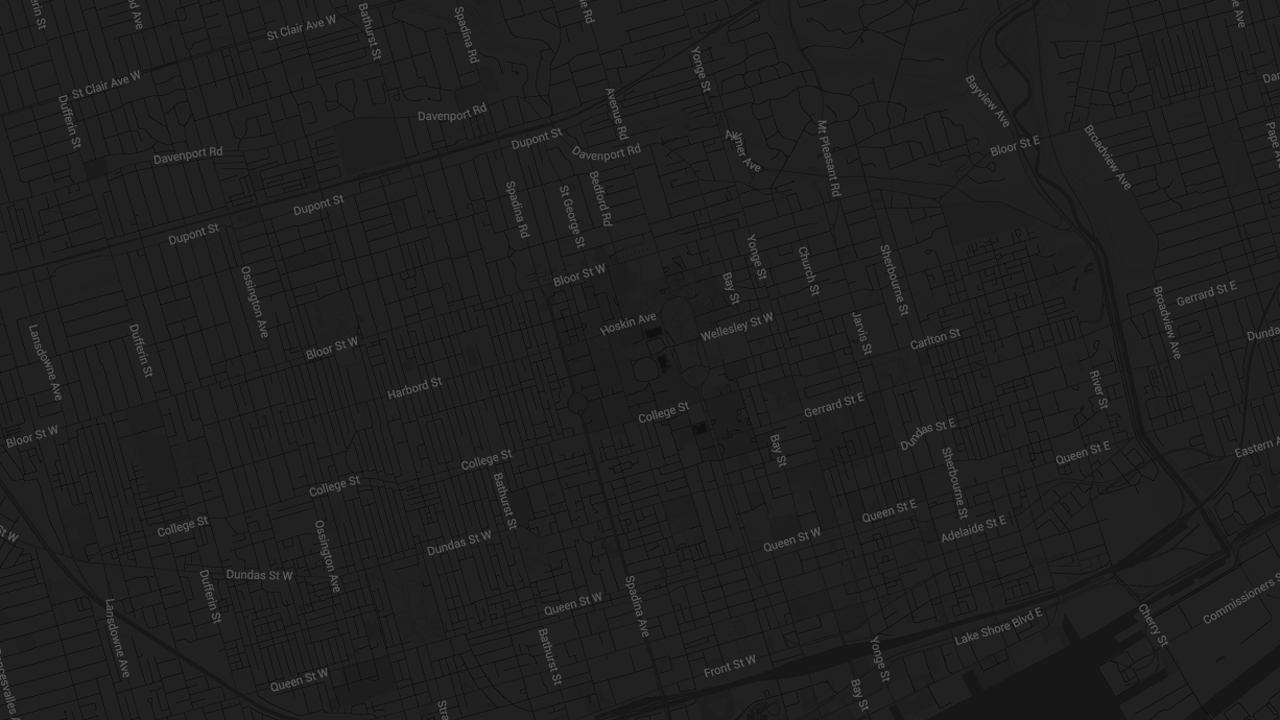
\includegraphics[scale=0.35]{figures/map-style.png}
    \caption{Map design for the Relay GUI.}
    \label{fig:map-styling}
  \end{centering}
\end{figure}

Following the development of map styling, a refinement of the data visualization and corresponding features of the application continued.
Figures \ref{fig:histo-1} - \ref{fig:dots-2} show multiple iterations of both the histogram and circular polygon overlay approaches to the design of the prototype.\\

\begin{figure}[htbp!]
  \begin{centering}
    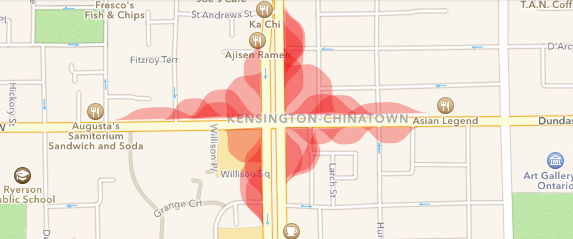
\includegraphics[scale=0.77]{figures/histo-1.png}
    \caption{Mid-fidelity histogram overlay design.}
    \label{fig:histo-1}
  \end{centering}
\end{figure}

\begin{figure}[htbp!]
  \begin{centering}
    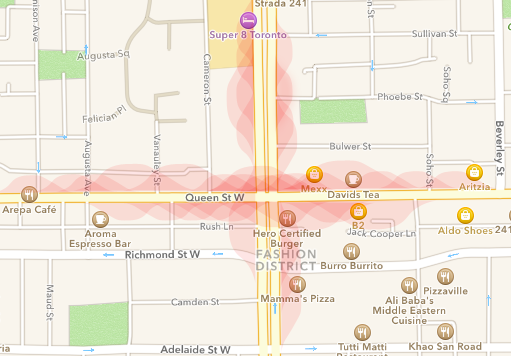
\includegraphics[scale=0.77]{figures/histo-2.png}
    \caption{A second mid-fidelity approach to histogram design.}
    \label{fig:histo-2}
  \end{centering}
\end{figure}

\begin{figure}[htbp!]
  \begin{centering}
    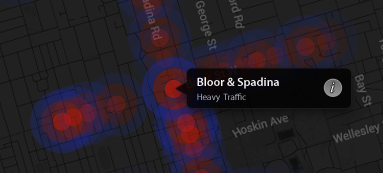
\includegraphics[scale=1]{figures/dots-1.png}
    \caption{Traffic data visualized as a heat map using a concentric circle approach.}
    \label{fig:dots-1}
  \end{centering}
\end{figure}

\begin{figure}[htbp!]
  \begin{centering}
    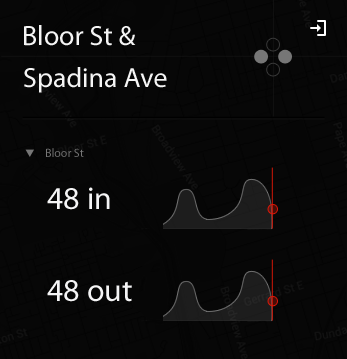
\includegraphics[scale=1]{figures/side-panel.png}
    \caption{Mid-fidelity design of a side-panel containing visualizations of traffic metrics.}
    \label{fig:side-panel}
  \end{centering}
\end{figure}

\begin{figure}[htbp!]
  \begin{centering}
    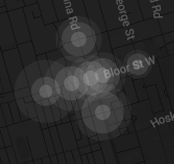
\includegraphics[scale=1]{figures/dots-2.png}
    \caption{A second mid-fidelity design for the concentric circle approach.}
    \label{fig:dots-2}
  \end{centering}
\end{figure}

Experimentation with colour, shape, and size was done during this phase, in order to optimize the pre-attentive processing and response from users, which when used correctly have been shown to trigger eye-contact and understanding within 200 - 250ms of viewing the graphic \cite{Healey93} \cite{Healey96}.
This is reflected in the various mid-fidelity iterations shown in the figures above.
Following this stage, the prototype moved into a high-fidelity phase, which involved finalizing interactions, visuals, and prototype features through the development of the prototype.\\

\subsubsection{High-Fidelity Prototype}

The design of the high-fidelity prototype took the lessons learned from each of the previous design iterations, and implemented them into a working Javascript-based web application.
This application - involving a custom-styled map, randomly generated traffic conditions for the city of Toronto, a side-panel for showing intersection data, and pop-up dialogues per intersection - was built using the circular polygon heat map approach for traffic visualization.
HTML and CSS styling was done to emulate and build out the mid-fidelity prototype design, and Javascript was employed to recreate the designed interactions to maintain a consistent and directed user experience. Screenshots from the high-fidelity prototype are shown below in Figures \ref{fig:screen-1} and \ref{fig:screen-2}. \\

\begin{figure}[htbp!]
  \begin{centering}
    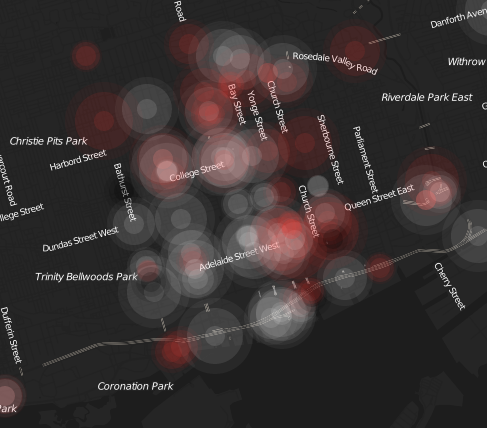
\includegraphics[scale=0.5]{figures/screen-2.png}
    \caption{Localized screenshot of a traffic cluster in the city of Toronto - from working prototype.}
    \label{fig:screen-1}
  \end{centering}
\end{figure}

\begin{figure}[htbp!]
  \begin{centering}
    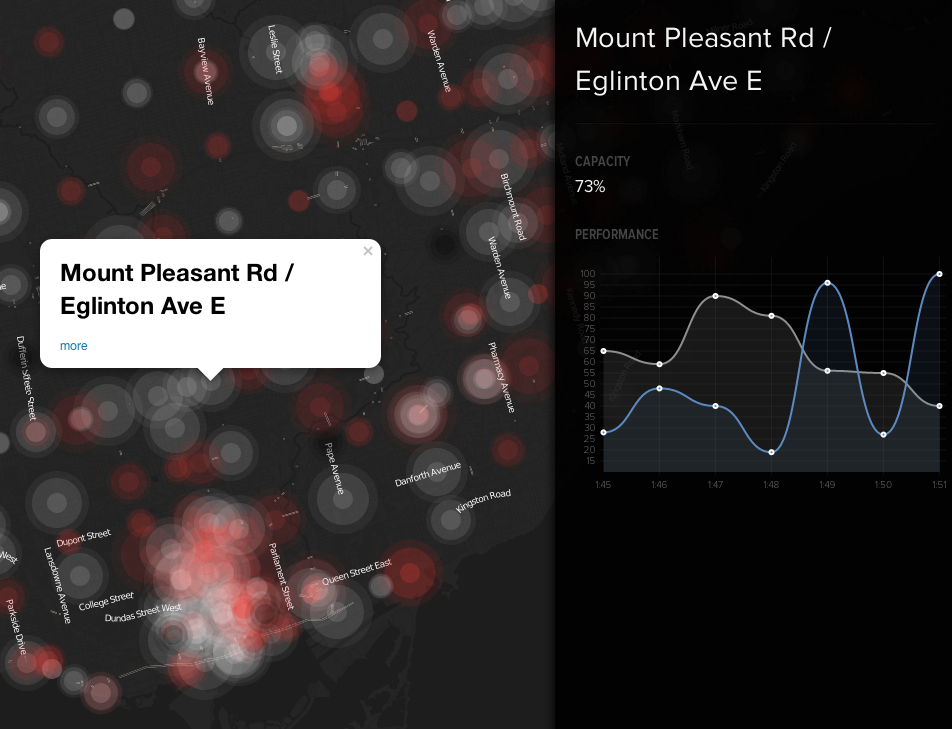
\includegraphics[scale=0.47]{figures/screen-1.png}
    \caption{Screenshot from working prototype showcasing popup menu, side panel, and graphical traffic data.}
    \label{fig:screen-2}
  \end{centering}
\end{figure}

Other interactions not shown include scrolling the page to zoom in and out of the map, as well as animation of the graph in the side panel to show real-time traffic updates.\\

\subsection{Back-End Design Approach}

The infrastructure powering the user-facing component of Relay is colloquially referred to as the ``back-end''.
The design goal for this particular component consisted of providing all the necessary resources to the client-side application with minimal development effort (effort that would otherwise be spent on more innovative areas of development).
Additionally, this layer acts as the \emph{glue} that holds together the Relay system.
This is outlined at a high level in a full system map in Figure \ref{fig:Back_end_system_map}.
The back-end exposes APIs required for the client-side application (front-end), as well as data processing and scheduling routines for the Relay Framework.
This component is characterized by an application server, database, and associated services (such as map tiling).\\

The core application framework was chosen based on familiarity and flexibility (rather than performance).
For this task the ``Flask'' python framework was chosen, as many team members had worked in this environment successfully in previous projects.\\

\begin{figure}[htbp!]
  \begin{centering}
    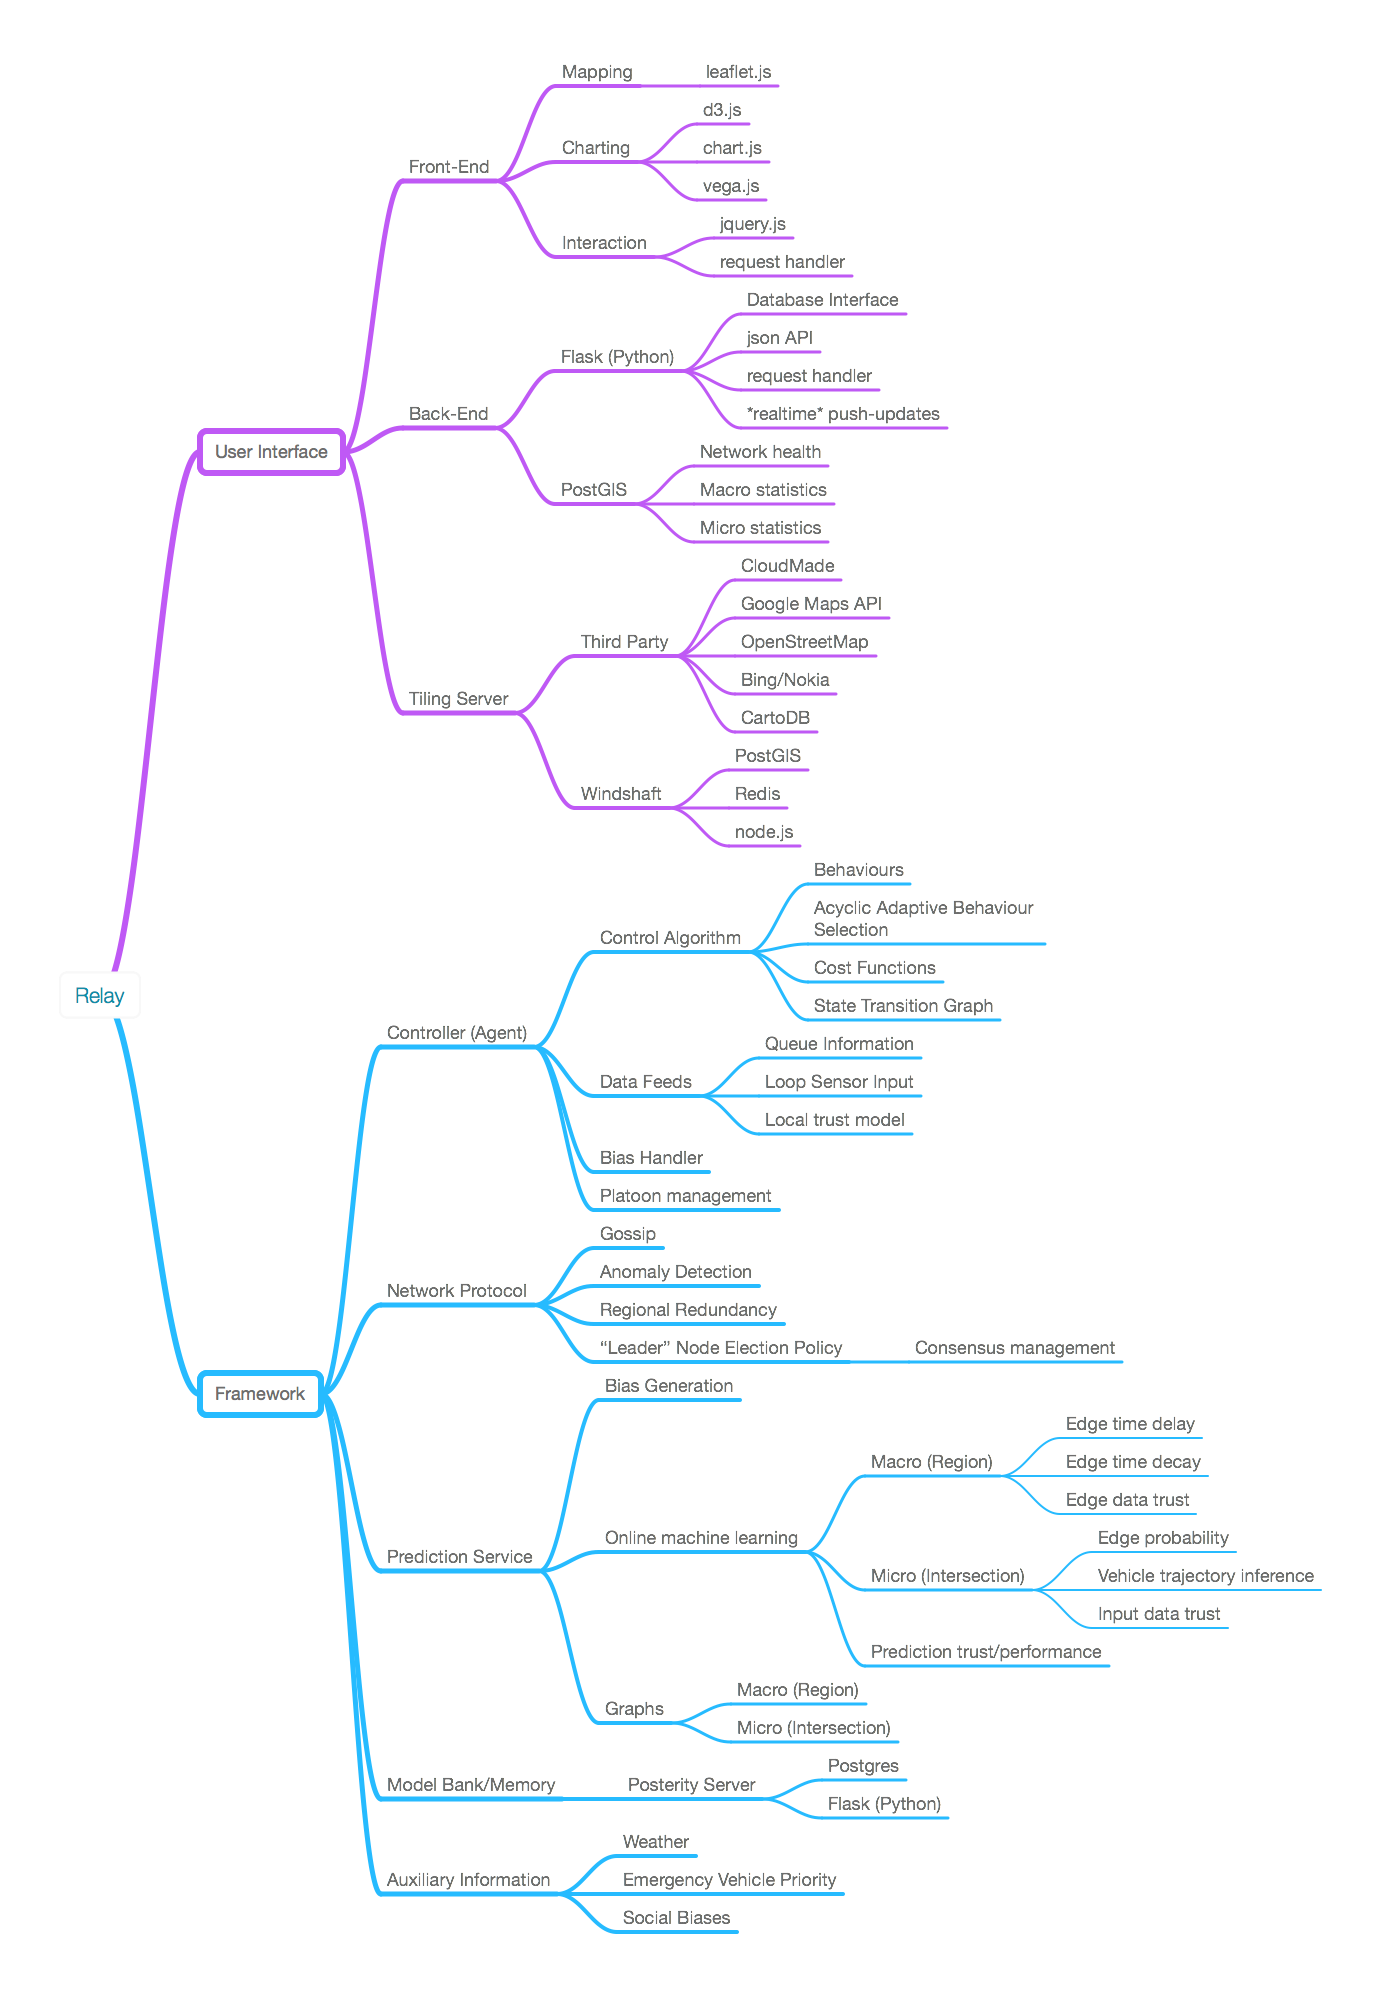
\includegraphics[scale=0.3]{figures/flow-chart.png}
    \caption{Relay: System Map}
    \label{fig:Back_end_system_map}
  \end{centering}
\end{figure}

Aside from the web-framework, the back-end design choices and technologies are broken up into modules.
To deliver the minimum viable product, the back-end must support online mapping via either a tile server or third party service, it must have some place to store various geospatial information (database), as well as some service to interface with the controller network (Relay Framework).
The various module design decisions and technologies selected are detailed below.\\

\subsubsection{Databases and Persistent Storage}

As with most applications, the Relay web-service requires some medium to safely and efficiently store structured data, the canonical use case of a database.
Database technology is highly mature, and for its ease of use, familiarity, and extensive documentation, additionally, many members of the team are familiar with SQL.
To capitalize on this, a SQL relational database management system was chosen to power the Relay iInterface.\\

The PostGIS (Postgres SQL, GIS package) database was chosen to power the geospatial aspects of the application.
PostGIS is industry standard, open source, powerful, extensible, and familiar - a natural choice.
SQLite3 was chosen as an auxiliary testing database for its simplicity: unlike Postgres, SQLite databases are contained entirely within a single file, and as such can be quickly and easily moved around the development environment (as well as captured by version control).
Postgres is not nearly so convenient, but dramatically more powerful, the postgresql database requires an operational postgres environment/server: additionaly overhead that was unnecessary for initial prototypes and designs.\\

\subsubsection{Mapping Support}

Online mapping consists of several components, the most visible of which are the map ``tiles''.
Tiles are canonically 256$\times$256 pixel images of geographical information that is rendered as a map at a specific zoom-level.
When a user interacts with an online map, they are presented with the illusion of one continuous (pannable, scrollable) image.
In reality, this effect is the result of some clever javascript on the client-side that renders individual tiles and moves them around in unison.
Building such a framework is outside of the scope of this design, however there exist multiple solutions in the market from third parties, as well as open-source alternatives.\\

Within the realm of online mapping, there are many high-quality, pseudo-differentiated products from many providers (the most prominent of which being Google, Bing/Nokia, and OpenStreetMap).
Within such a competitive market, there are many features available for comparison.\\

For our choice of tiling service (or ``map provider'') we valued the optimal combination of ease of implementation, and extensibility.
While not rigorously defined, the concept of extensibility allows us to change/reverse decisions with minimal cost later on (when we are better informed).
Additionally, highly flexible map providers are desired over proprietary solutions that limit extensibility options to within a single domain: Google, and Microsoft's services are examples of this.
In this case, the use of industry standard tools that can be adapted to an arbitrary mapping infrastructure (such as leaflet.js) is a benefit.\\

For full-scale applications, many of the third party services are not free (such as Google, Bing, OSM), this was not a deterrent for us as every provider evaluated offered free developer usage, however the extent to which this was offered varied dramatically.
Furthermore, in the interest of developing a highly \emph{democratic} adaptive traffic control framework, open-source technologies were preferred whenever available.
For example, WindShaft is a tiling server/cache that is built on entirely open-source technologies.
Windshaft is used explicitly by both CartoDB and MapBox.
Thus while we could assume the burden of running a Windshaft server, it is dramatically simpler in the short-term to take advantage of a third-party's Windshaft instance.\\

\begin{longtable}{|p{2.6cm}|p{2.1cm}|p{2cm}|p{2cm}|p{2.8cm}|p{2.8cm}|} \hline
    \textbf{Attribute}                        & \textbf{Google/Bing}            & \textbf{WindShaft}         & \textbf{CloudMade (OSM)}                 & \textbf{CartoDB}               & \textbf{MapBox}               \\ \hline
    Free Plan Restrictions (tiles) & within reason          & n/a               & 500k                            & 750k                  & 45k (no satellite)   \\ \hline
    Database Restrictions            & none                   & none              & none                            & 50MB/10 tables        & 50MB                 \\ \hline
    Standard API (leaflet.js)        & Proprietary            & lealet.js         & leaflet.js                      & cartodb.js/leaflet.js & mapbox.js/leaflet.js \\ \hline
    Themes/Style                     & specialized JavaScript & css/mss           & style-wizard (not configurable) & css/mss               & css/mss              \\ \hline
    extensibility                    & Within Google Apps     & open-source (yes) & unknown                         & open-source           & partial open-source  \\ \hline
    \caption{Feature Comparison of Mapping Service Providers}
    \label{tab:Map_Provider_Attributes}
\end{longtable}

The choice of mapping provider was relatively straightforward according to the following criteria:\\

\begin{longtable}{|l|l|} \hline
    \textbf{Attribute}              & \textbf{Criteria}            \\ \hline
    Free Plan Restrictions & Higher is better    \\ \hline
    Database Restrictions  & Less is more        \\ \hline
    Standard API           & Must use leaflet.js \\ \hline
    Extensibility          & Higher is better    \\ \hline
    Themes/Style           & CSS/MSS is better   \\ \hline
	Initial Expense        & Lower is better	 \\ \hline
     \caption{Mapping Service Selection Criteria}
     \label{tab:Map_Selection_Criteria}
\end{longtable}

Due to the qualitative nature of our requirements, a lot of weight was attributed to tiling services/interfaces that involved making the minimal upfront commitment.
For example, running our own Windshaft server gives us the most control and flexibility (and may be what ends up powering the final prototype), but it requires a significant investment in time at the beginning (such as setting up a redis server, database, and associated node.js application) time that isn't necessarily budgeted.
Windshaft is a mature open source platform for geographical tiling, and powers CartoDB, MapBox, and many other modern third party mapping services.\\

For the initial prototype, the CloudMade service was used to power the Relay mapping service.
Due to no coupling of the GIS database and the mapping service, explicit use of leaflet, and high similarity to the \emph{ideal} windshaft implementation, but available instantly with very little developer overhead the OSM-powered CloudMade mapping service was a natural choice.
One significant downside of the CloudMade offering is the relative lack of control over the map tile styles.
Modern platforms such as MapBox and CartoDB allow full customization of the map styles through the use of configuration/style files that offer complete control over the style/colouring of arbitrary map tiles at arbitrary zoom levels.
This includes physical and cultural geographical information (such as street labels as well as rivers etc.).
This is a byproduct of their usage of WindShaft under the hood, which offers these features.\\


\subsubsection{Data Processing Service}

The second major component of the back-end involves interfacing with the Relay Framework.
The presentation of geospatial statistics and related traffic performance metrics associated with or surrounding each individual agent is a requirement for the Relay Interface, and as such a dedicated module is needed to collect and structure information sourced from the Agents.
Currently this module is not a component in the low fidelity prototype as the necessary infrastructure (i.e. a network of Agents) has not yet been implemented.
However, the goal of such a system is to acquire the necessary information from the Framework while minimizing the computational and network load on the individual controllers.
Using the Flask framework, the service will likely consist of a lightweight service that exposes a JSON API similar to the interface provided to the client-side application.
Initial implementations will involve naive \emph{polling} methodologies; in which the web service periodically refreshes itself by requesting new information from the Relay Framework.
Development resources will likely be spent on the Relay Framework itself to allow for efficient access.
For example, if the Relay Agents each contain semi-redundant information about traffic patterns, it is not necessary to individually scrape all intersections in the network to receive updated data.\\

\subsubsection{Testing Methodology}

As the intermediate layer between the Relay Framework, and the Relay Interface, the back-end performs little in the way of computation (other than ETL associated with communication).
Thus the main requirement (excluding the map/tile service) is to respond to requests from the Relay Interface promptly.
Noticeable lag between modules, especially as it relates to the interface can dramatically reduce the end-user experience.
While this may not be of paramount importance for prototyping, it does become useful during development, and is further exacerbated by our technological constraints (hosting the platform locally on our personal computers).\\

That said, within the realm of software development there are a large battery of tests/testing-related-philosophies that could see application within this project.
At the highest level, system integration tests will be used to ensure platform robustness, especially in development.
At the code module level, the typical suite of unit tests will be used to assert correctness.
However, due to time requirements, rigorous testing is neither wanted nor warranted, and as such only the most critical systems will be tested in this way.
For example, the request handler is invoked every time the Interface needs new information, this module should be exceptionally robust to failure.
In a similar fashion, database connections can involve a significant amount of complexity if handled poorly.
Within this respect we follow the motto that the architecture should guide development to reduce the likelihood of system failure.
In this string, we have endeavoured to architect the Relay system as multiple pseudo-independent modules, each with their own functional (correct) core.
This design pattern is commonly referred to as ``Ports and Adapters'' or ``Hexagonal Architecture''.\\

\subsection{Design Approach for the Relay Framework}

Real-time, distributed traffic control is an interesting problem, with many creative solutions.
The modules and operators that handle individual intersection signal timing, data collection and backup, and statistical modelling, as well as the network topology that holds it all together is brought under the umbrella term ``Relay Framework''.\\

The goal of the framework is to address the intelligent traffic control problem from the \emph{bottom-up}.
Within the framework, each intersection is endowed with its own autonomous signal timing controller or ``Agent''.
In isolation, each Relay Agent seeks to maximize intersection throughput (as measured through various arbitrary metrics) subject to local environmental/contextual constraints.\\

\subsubsection{Relay Intersection Modelling}

In general, any intersection in Relay can be modelled as a graph (physically this is also the case).
Intersections in Relay are modelled as directed acyclic graphs, where each inlet and outlet are distinct nodes/vertices, and the edges are legal paths that a vehicle could follow to get from one inlet to a corresponding reachable outlet.
Each edge in the graph (aside from containing reachability/adjacency information) contains probabilistic information pertaining to that particular physical path.
This is shown in Figure \ref{fig:Relay_Intersection_Graph}.
At the highest level, the Relay Agent, in conjunction with its local prediction service learns a probability for each edge, which represents the liklihood that a vehicle will choose to traverse that given edge if it arrives at the originating inlet.
For example, in the case of an intersection with a dedicated left turn lane, the associated edge would have a probability of 1, meaning we would expect that all vehicles who enter the left-turn inlet, proceed to execute a left turn.
It also follows from this that the sum of out-going edge weights for a given inlet will always be one.\\

\begin{figure}[!ht]
	\caption{Relay Intersection Graph Model}
	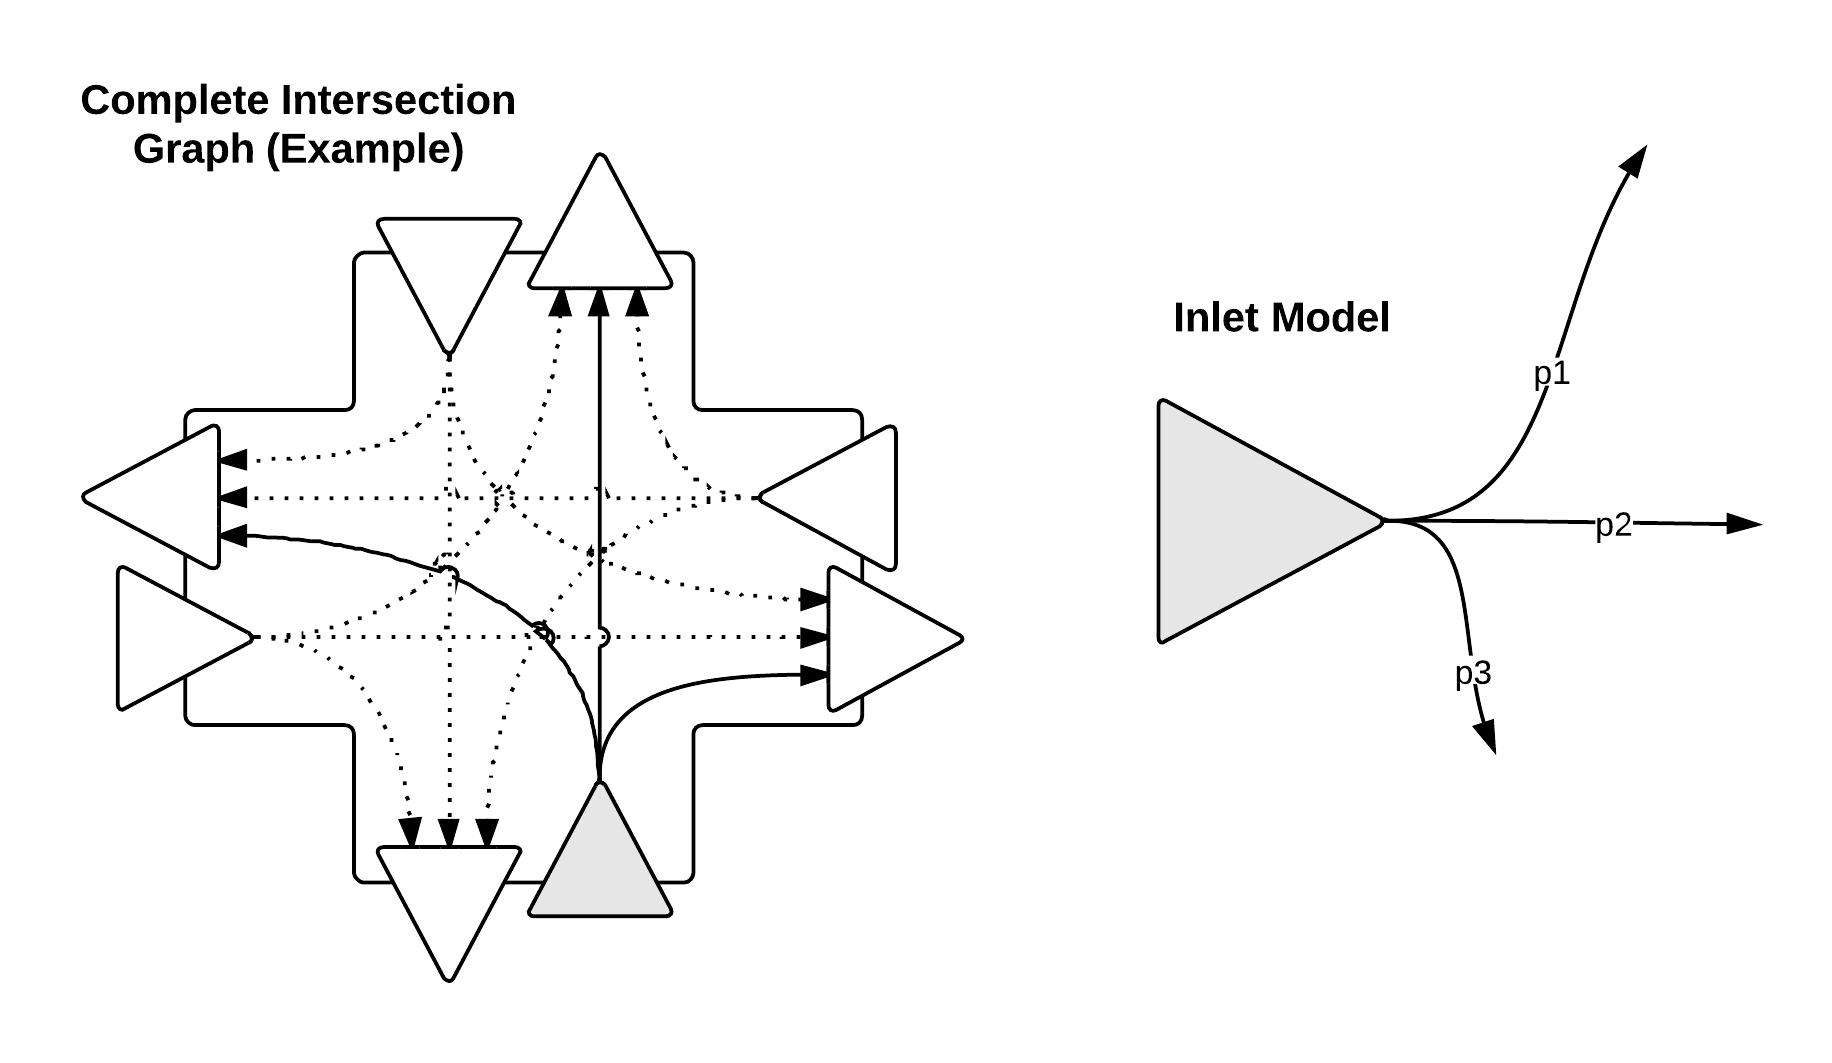
\includegraphics[width=\textwidth]{figures/Relay_Intersection_Graph.png}
	\label{fig:Relay_Intersection_Graph}
\end{figure}

Similar to the complete intersection graph, legal signal states (i.e. Green vs. Red lights) are also described as a graph.
These \emph{Behaviours} are subgraphs of the complete intersection graph, with similar properties.
Thus each behaviour describes a discrete number of inlets (and associated outbound edges) to serve at a given time, in this manner Behaviours can be chosen (by the controller) to serve the inlets that best maximize short-horizon flow.
Additional information regarding this process is discussed in the ``Relay Agent'' section below.\\

\subsubsection{Relay Agent}
The Agent module contains all the necessary ingredients for soft-real-time acyclic reactive adaptive signal timing.
An outline of the Agent module is contained in Figure \ref{fig:Relay_Agent_Controller}.
The controller is set up as a maximization process which weighs the current and predicted traffic profile (as well as queue statistics if they are available) and selects the appropriate \emph{behaviour} to optimally fulfill its objective function.\\

\begin{figure}[!htpb]
	\caption{Relay Agent Controller}
	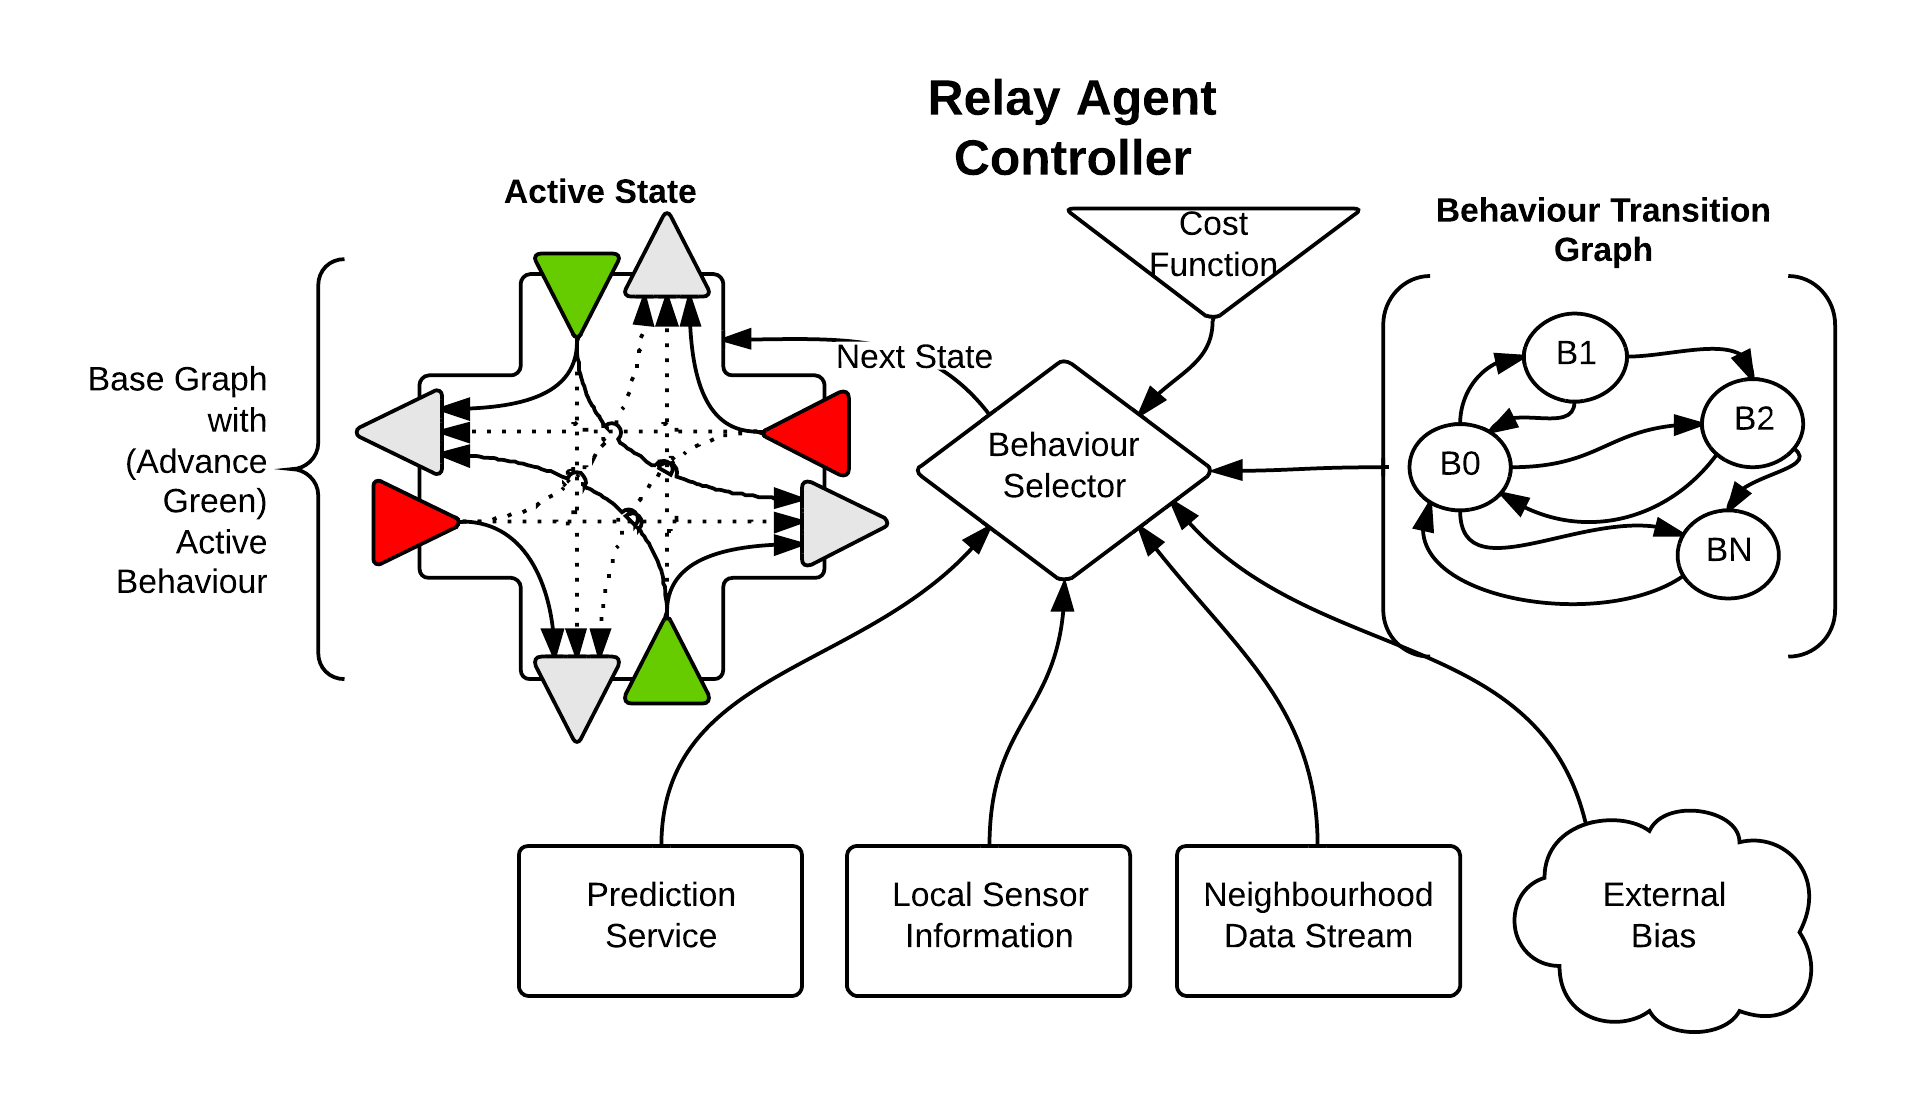
\includegraphics[width=\textwidth]{figures/Relay_Agent_Controller.png}
	\label{fig:Relay_Agent_Controller}
\end{figure}

Similar to the Relay Intersection model, the behaviour transition graph (or matrix, depending on the implementation) contains information related to the cost associated with changing the current signal, as well as logistic information such as minimum behaviour durations.
Where signal behaviours are encoded as nodes/vertices, transition costs (dead time, minimum signal duration, vehicle lag, etc.) are among the edge properties.\\

For example, switching the direction of traffic flow cannot be done instantaneously, furthermore in most countries there is a minimum amount of ``red'' time that must be allocated in both directions to allow lagging traffic to safely exit the intersection.
Thus the amount of time required to switch a particular signal behaviour depends on the current state of the intersection.
As another example, consider the concept of an \emph{advance-green} a behaviour typically following ``red''-time favouring a particular direction, granting vehicles wishing to turn left right of way for an arbitrary amount of time.
In Relay, this advance green signal is treated no differently from any other signal behaviour.
In this case the associated transition cost to switch behaviours from advance green to \emph{full} green is very low.
This information is encoded in the edges of the behaviour transition graph.\\

Aside from dictating the signal behaviours and durations, the Agent is also responsible for updating its internal intersection probabilities, and processing/interpreting local traffic sensor data.
It is important that in the scope of this project, we have assumed we have \emph{perfect} traffic data at the intersection level.
We acknowledge that this is a large assumption that is not necessarily realistic most traffic systems have notoriously poor sensing capabilities \cite{Miovision:2012}.
However as a matter of scope, many companies (such as the Kitchener-based Miovision) have commercial solutions to this problem.
As a coping mechanism, it may be possible to leverage the Relay prediction service to develop an internal \emph{trust} model associated with each intersection's sensors.\\

\subsubsection{Network Topology}

To a particular Agent, the Relay Framework appears as a mesh network centred around it.
The choice of network topology was not difficult given our design constraints (for the Framework) include a high degree of fault tolerance, robustness, and physical distribution.
Peer-to-peer (p2p) Mesh network topology (aside from being relatively novel) is a natural fit for these kinds of constraints.
Particularly as many of the technology's weaknesses (poor latency, poor scaling behaviour for complete connectivity of all Agents, etc.) are explicitly avoided by the Relay Framework Architecture.\\

In traditional Mesh Networks, each node is tasked with repeating the messages of other nodes to its neighbours/peers.
This results in a lot of overhead for individual nodes.
Within the Relay Framework, Intersection Agents do not require an active connection to every other Agent in the network, they only care about their immediate (or to some finite-depth) neighbours.
This depth-wise priority is shown in Figure \ref{fig:Relay_Network}.\\

\begin{figure}[!htpb]
	\caption{Relay Network Neighbourhood}
	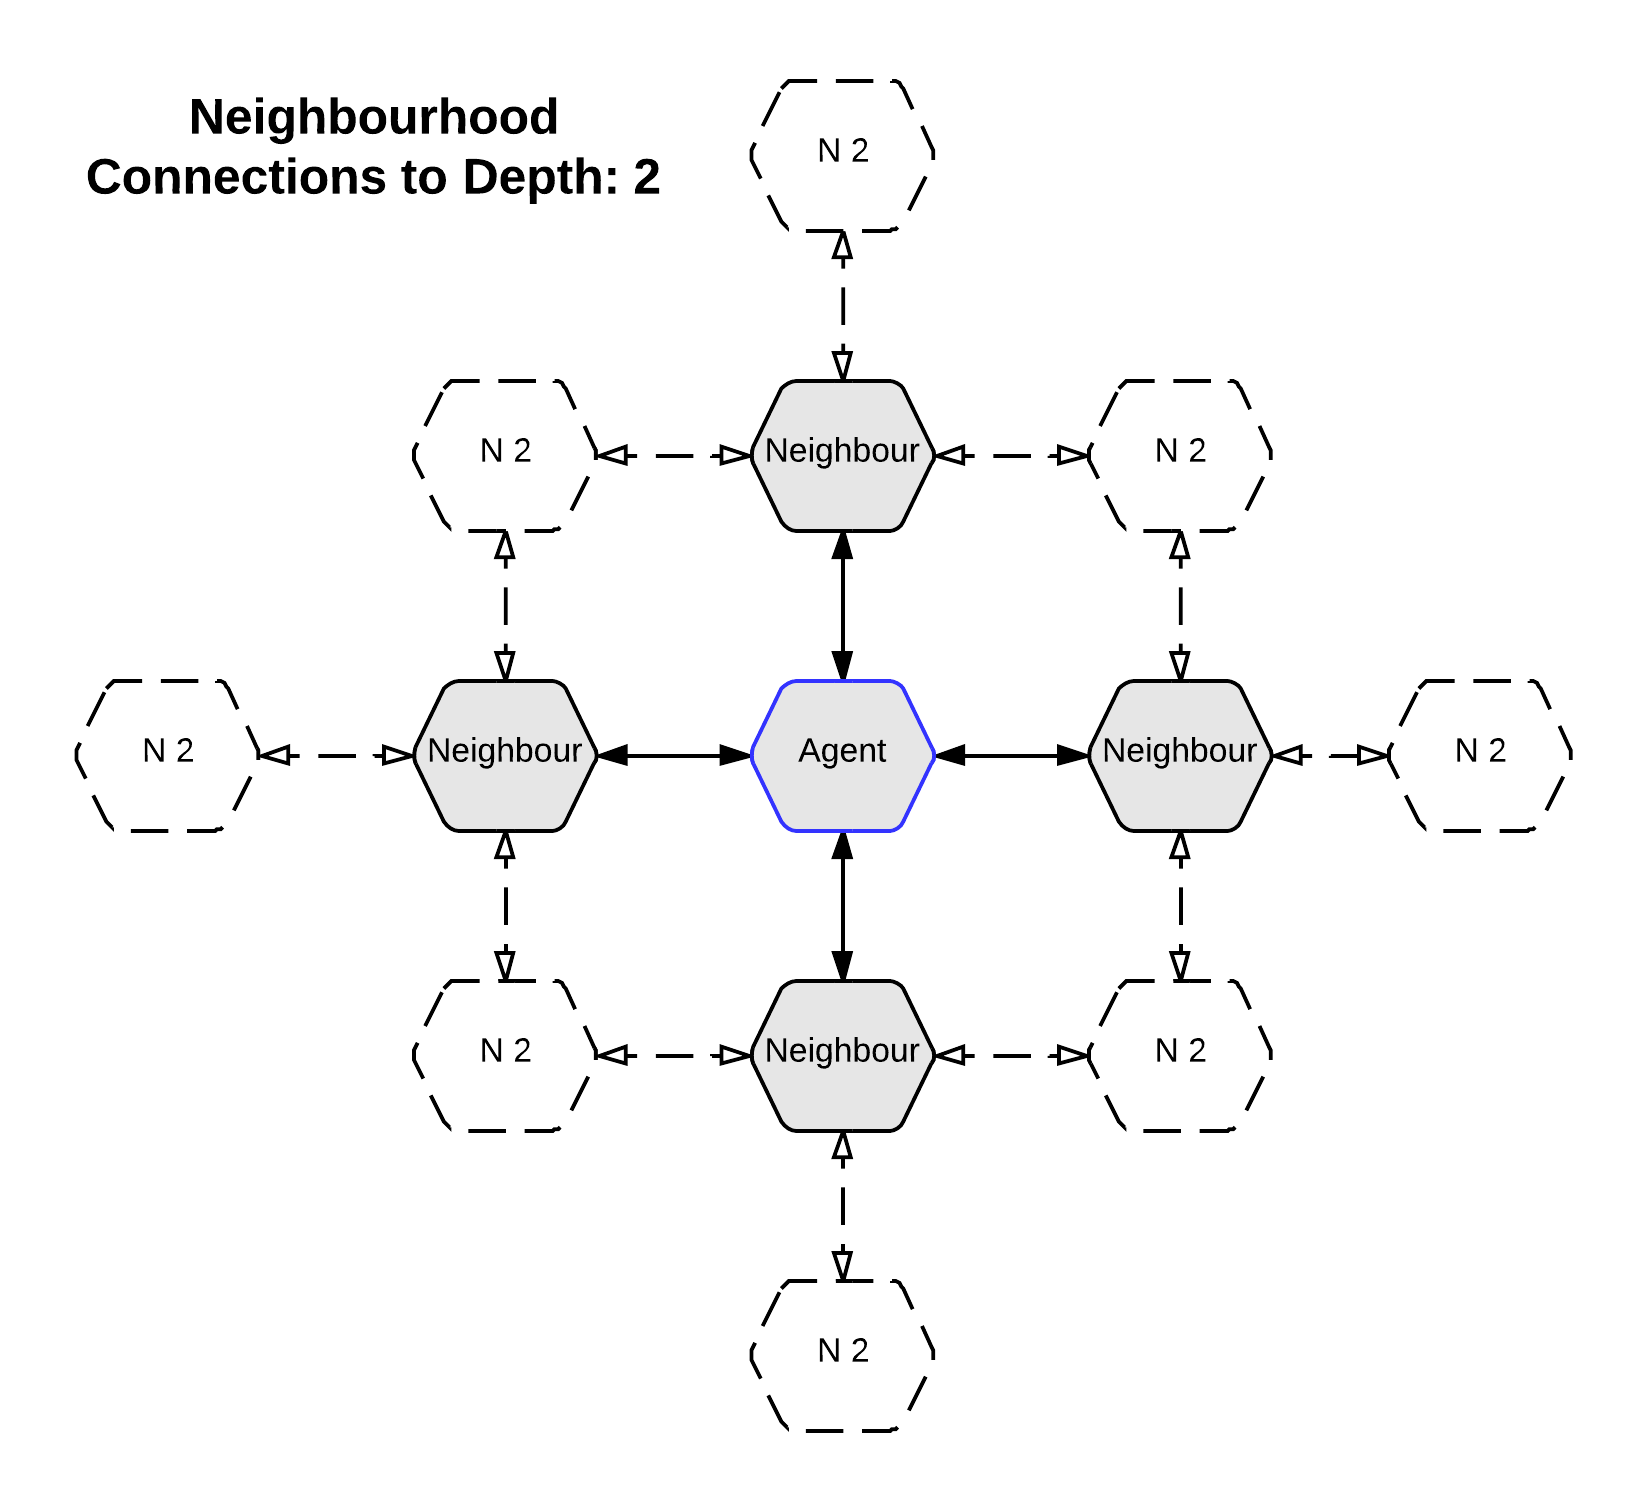
\includegraphics[width=\textwidth]{figures/Relay_Network.png}
	\label{fig:Relay_Network}
\end{figure}

Alternative network topologies have been used by current adaptive traffic implementations.
For small scale (arterial) installations, it is trivial to have all agents permanently connected to all peers.
Modern installations have also implemented so-called ``cloud-service'' based approaches, and Miovision's Spectrum is one such example.\\

\subsubsection{Scope of Prediction Service}

One of the main design features of the Relay Framework is the ability to apply generalized graph-predictive statistical methodologies to arbitrary signals.
The most visible of which at the local level are the path probabilities within the intersection these are used to optimally select and transition between behaviours.
However, this core service is also applied at the macroscopic, or neighbourhood/regional scale.
This is outlined in Figure \ref{fig:Relay_Macro_Graph}.\\

\begin{figure}[!htpb]
	\caption{Relay Macroscopic Information}
	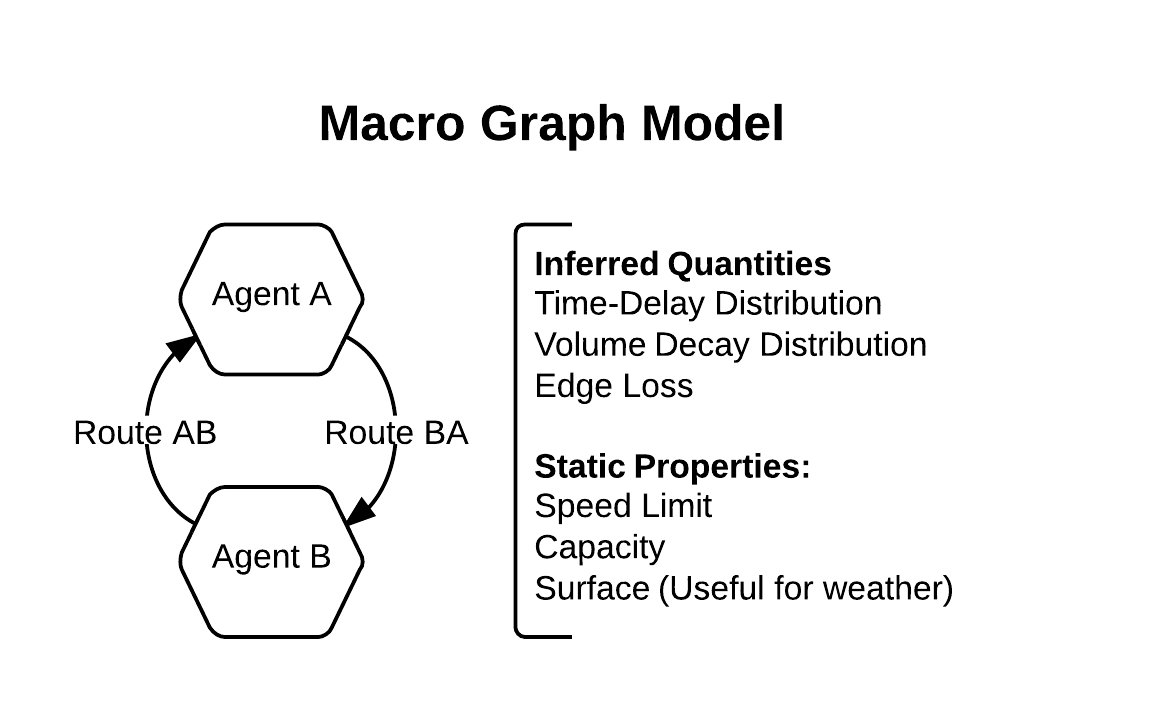
\includegraphics[width=\textwidth]{figures/Relay_Macro_Graph.png}
	\label{fig:Relay_Macro_Graph}
\end{figure}

\subsubsection{Exploiting Neighbourhood Redundancy}

The implementation of a final proof of concept contains many interesting research, design, and implementation challenges.
One such challenge is optimizing network communication within the purview of the neighbourhood mesh network topology.
While not a primary concern of this document or project, it is mentioned here for completeness and as a possible stepping stone for further research.\\

As was mentioned in the discussion on network topology, and hinted at in Figure \ref{fig:Relay_Macro_Graph}, multiple agents will have very similar information about each other.
It is possible to exploit this redundancy to efficiently store copies of network-wide data either for posterity or to introduce more convenient mechanisms to access the information.
An example of such a use-case is the Data Processing module within the Relay Back-end system.\\

Similar to raft-consensus models, we plan to introduce a distributed ``Super Node'' selection policy within the network.
Such a policy entails the Agent network to elect (from their own ranks) a \emph{Super Node} to act as a data uplink to external services for particular pieces of data.
For example, in the case of a neighbourhood of Agents, the region can elect a member (perhaps based on hardware capability, stability, trust, or other metrics out of the scope of this project) to act as the external point of contact or liaison for external services wishing to access the network data.
Similarly, these Super Nodes would be allowed to break the \emph{network depth} requirement enforced by our network topology, and communicate/subscribe to other Super Nodes.
Network updates could be pushed externally to a single Super Node, which would be responsible for gossiping the update to its peers, and neighbourhood.\\

\subsection{Test Procedures}

The dynamic traffic control system will require training to develop a model from which it will attempt to optimize traffic flow.
Traffic and multi-agent simulation softwares exist which simulate traffic networks and allow for the application of traffic loads on said networks.
The dynamic traffic control system can be connected to the software to understand and control the simulated traffic network.
This will be used to train the dynamic traffic control system to optimize traffic flow.\\

Because the system's performance is dependant on the specific nature of the traffic network being used for simulation, performance must be measured with respect to alternative systems on the same traffic network.
Alternative models will be developed to benchmark the solution's performance.
First, a static, centralized control system will be developed based on basic traffic flow principles to control the system.
This will stand as a core benchmark for traditional traffic control systems.
In addition, a basic dynamic traffic control system will be developed as a more legitimate performance comparison.
The system will utilize basic features of a dynamic traffic control system, such as a distributed control system and dynamic traffic flow optimization.
The purpose of this benchmark is to highlight the advantages of the developed system to what is currently considered modern in research and industry.\\

Using the aforementioned traffic simulation software, the three models will be run through a series of performance tests.
Due to the chaotic nature of traffic simulation, multiple trials will be performed for each test, and means will be used for comparison.
First, the models will be given a constant traffic volume for an extended period of time.
This will allow us to understand how well the system is able to optimize traffic flow under ideal conditions.
Second, the models will be tested with surge simulations.
This more accurately models traffic flow, particularly in urban areas where morning and afternoon traffic surges are caused by commuting populations.
Finally, models will be tested in the presence of external disturbances.
Situations such as local power outages and emergency road closures will be simulated in both constant and surge traffic scenarios to measure the impact on the system.
From these observations, changes to the behaviour of actors in these situations can be adjusted to provide a better result.\\

Lastly, software unit and system testing will need to take place to ensure the system is stable and all functions work properly.
These tests will cover all major functionality in the system and assist in identifying issues.
While this does not directly impact a specific objective, it is a necessary step to meet each of the objectives.
If the software is not stable, catastrophic failures could occur and render the system unusable and potentially dangerous.\\

\section{Financial Budget}

The current scope of the project requires no physical components to be purchased, and no special facility space will be required.
There are no costs (other than developer time) associated with the research and development phases of this project.
Research material will be obtained through the university at no charge.
Personal equipment will be used for all software and algorithm development. Special software required for modelling or testing will be obtained at no cost through the University by donation from academic advisors.
Small-scale performance testing can be run on the team's personal or auxiliary computers.
Large-scale testing may require enhanced computer performance, for which time on more powerful server resources will be purchased.
The use of traffic models for real cities would provide a more compelling understanding of the benefits of our system.
Attempts will be made to obtain traffic data for existing cities for use in simulations.
In lieu of this, simulated traffic data will be used.\\

\newpage
\section{Project Progress and Schedule}
This section contains information regarding the current state of the Relay implementation, prototypes and designs.

\subsection{Review of Progress}

Overall the progress this term has not exactly aligned with what was projected.
The team has spent more time than anticipated discussing and devising methods for tackling the problem.
The specific areas that required extra planning are: architecture and features of intersections, construction of intersections and behaviours, and tools needed for visualizing.
We spent considerable time planning and discussing how to best understand an intersection's operation and construction, which helped us better grasp what needs to be created.
A lot of time and effort was spent acclimatizing to the current state of the art research in the field of traffic engineering and control.
However, it is expected that this contextual awareness will yield a more performant and relevant proof of concept.\\

Also, the simulation environment that was going to be used, Vissim, did not contain the features the team needs.
It is difficult to programmatically interface with this application and would be very tedious to create simulations by hand.
Each road piece, intersection, and parameter needs to be created by hand, which would be too time consuming.
Therefore, the team must either spend time creating basic simulations with Vissim, continue looking for other solutions, or create our own.
The team proposes using a combination of these tactics to suit the state of the project; Vissim may be helpful in early prototyping, but not large-scale simulation.\\

Next, after reviewing the goals in detail, the team believes that they may have been too ambitious.
Without much background in the types of systems that will be created, we underestimated the time required to research, plan, and create the solution.
The goals have been revised and are reflected in the Tasks and Deliverables section below.\\

Additionally, more research than expected was put into finding the right tools to make development easier.
Multiple mapping and rendering tools were tested and prototyped to determine which would satisfy our needs.
This slowed down development of the application and a new timeline for this has been set out in the section below.
Now that there is a foundation for the interface development speed should increase substantially and goals have not been adjusted (but have been modified to reflect changes we are making to the application's functionality).\\

Lastly, the team decided that a full Quartz Composer model would not be needed.
Due to time restrictions, this process would take too much time and therefore we will simply iterate designs in the application itself, but will still use Quartz models when useful.\\

The following section discusses how we will work to mitigate any deviations from the proposed timeline.
While we did not make as much progress as anticipated in the Fall term, the team is confident that we will be able to accomplish what is specified in the revised timeline.\\

\subsection{Strategies for Improved Performance}

To mitigate these issues the team has decided to schedule more frequent brainstorming and work sessions.
While there were ongoing sessions throughout the term, increasing this number will be necessary to complete the proposed design.
This is not included in following sections, but the team proposes a weekly, or twice weekly when permitted, development meeting to work through issues together.
We will also work on tasks individually, but this will be an opportunity to collectively work through problems and maintain higher focus by having scheduled work time.\\

Additionally, the team attempt to utilize our supervisor, and his resources, more frequently to gain more insight from him.
This should help with overcoming roadblocks that we encounter and improve our final solution.\\

\subsection{Tasks and Deliverables}

Below is an overview of the tasks to be completed over the Winter 2014 term.
These outline the major milestones and steps that will be taken to create the final prototype, presented at the final symposium.
The description column goes into detail about what will be performed in this task, and in many cases describes what will be included in that tasks deliverable.
The deliverable column, where applicable, identifies the high-level product of each specific task.\\

\begin{longtable}{|p{4.5cm}|p{6cm}|p{4.5cm}|} \hline
    Task                                              & Description                                                                                                & Deliverable                           \\ \hline
    Team Debrief, Update (W1)                         & After the Holiday's team will meet over the first few weeks to get back up to speed with what was accomplished the previous term and over the break as well. Will begin creating a detailed list of tasks to be completed.         & N/A                                   \\ \hline
    Response to Feedback (Jan 21)                     & Details of this report TBD                                                                                                                                                                                                         & Report                                \\ \hline
    Meet with Supervisor (W2)                         & Meet again with supervisor to discuss our progress and plan. Get his insight on our solution/plan/etc. and input on what we could change or improve.                                                                               & N/A                                   \\ \hline
    Actor Development and Research (W2)               & Continue building functionality of ``actors'' (i.e. intersections). Begin development of network architecture (how do you connect all actors together?). Further research of programming paradigms required to construct the system. & Architecture designs and construction \\ \hline
    Application Development (W2)                      & Continue iterating on current interface/interaction design. Add more features (e.g. advanced traffic information panel) and incorporate newest functionality from back-end.                                                        & Updated interfaces and application    \\ \hline
    Network Development (W3-W4)                       & Ability to set-up a network of actors, actor functionality established, and actors able to ?talk? to each other.                                                                                                                   & Passes unit tests                     \\ \hline
    Online Predictive Model Prototyping (W4-W5)       & Begin prototyping algorithms for controlling the network. Will utilize knowledge gained from researching other systems and reading papers on current state of the art.                                                             & Direction to proceed with algorithms  \\ \hline
    Small Network Trials (W4 - W5)                    & With algorithms, perform tests with a small network of actors (e.g. 2-5 nodes). Iterate on designs as needed. Also, connect with front-end to test data streaming capabilities.                                                    & Passes network tests and benchmarks   \\ \hline
    Update Meeting and Simulation Research (W4/5)     & Meet with supervisor to discuss current progress. Bring up any difficulties we are having and work through these. Continue investigating simulation environments. May revise timeline after decision about this is made.           & Simulation environment understanding  \\ \hline
    Prototype Update Demo/ Feedback (Jan 31 - Feb 11) & Present updated prototype. Show current progress and gain feedback from peers. Make changes to solution based on this where needed.                                                                                                & Feedback, Presentation                \\ \hline
    Online Predictive Model Development (W5 - W6)     & Based off prototype and testing conducted, formalize the algorithms to be used in traffic control. May updated after large-scale network tests completed                                                                           & Passes network tests and benchmarks   \\ \hline
    Application Development (W6)                      & Continue adding features to the interactive application. Integrate more features with back-end                                                                                                                                     & Refined application experience        \\ \hline
    Larger Network Tests (W6 - W7)                    & With algorithms, perform tests with a larger network of actors (e.g. \~50-100 nodes). Changes to model will be made based on the results of this.                                                                                  & Passes network tests and benchmarks   \\ \hline
    High-Fidelity Model Development (W7-W8)           & Continue adding features to algorithms, improving stability, testing network, and providing information for front-end                                                                                                              & Passes unit tests                     \\ \hline
    High-Fidelity Application Development (W7-W8)     & Finish developing application. Test all functionality to ensure it meets the goals.                                                                                                                                                & Passes unit tests                     \\ \hline
    Final testing (W8-W9)                             & Testing of sim-env and system for prototype demo. Fix any issues that arise.                                                                                                                                                       & Passes unit tests                     \\ \hline
    Symposium (Mar 14)                                & Team will present the prototype that has been created. Will identify challenges that arose, what modifications needed to be made, and how goals were met or revised.                                                               & Demo, Slides, Presentation            \\ \hline
    Project Video (Mar 25)                            & Details TBD.                                                                                                                                                                                                                       & Video of project                      \\ \hline
    Final Submission (Apr 4/8)                        & Completion of all deliverables.                                                                                                                                                                                                    & Report, logbook, etc.                 \\ \hline
    Outreach Presentation                             & Completed in Fall 2013.                                                                                                                                                                                                            & Presentation, summary                 \\ \hline
\caption{Tasks and Deliverables}
\label{table:tasks-deliverables}
\end{longtable}

\newpage
\subsection{Gantt Chart}
\begin{figure}[htbp!]
  \begin{centering}
    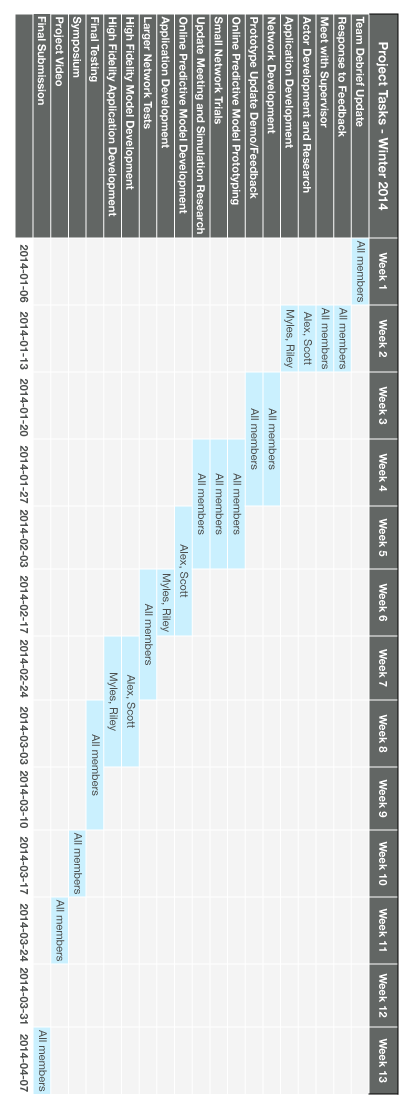
\includegraphics[scale=0.5]{figures/gantt-vertical.png}
    \caption{Gantt Chart for Winter 2014}
    \label{fig:gantt}
  \end{centering}
\end{figure}

\newpage
\section{Conclusion}

Over the last decade there has been a resurgence in interest surrounding intelligent traffic control systems as the burden of congestion in urban centres has continued to increase.
Relay proposes to attack this problem from two angles: providing transparency to the traffic network, and providing a platform for sophisticated agent-based control mechanisms for adaptive signal timing; yielding the Relay Interface and Framework respectively.\\

The Interface includes detailed metrics regarding traffic flow and provides insight into transportation network performance for both traffic engineers and the general public.
The Framework will be constructed in two parts (network and algorithms), acting as the brain of the system.
The network will consist of independent agents that interface and communicate with each other to share up-to-date information and predictive models.
The algorithms will sit on top of this layer and will make decisions about signal timing, behaviours, and overall traffic flow.
Information, statistics, and a queriable interface will be shared between the front- and back-end to provide greater transparency to users of the system.\\

Relay is a proof of concept for a democratic, distributed peer-to-peer intelligent traffic control system, and associated open data initiatives, thus it is important to note that the team is approaching this as a research problem and as such, creating sustainable business (while enticing) is not a priority.
The main goal is to push the envelope of the state-of-the art in ATCS, which in many scenarios involves flouting the current commercial implementation methods and models.
 We will incorporate leading traffic control research with our proposed framework, and combine it with interesting, understandable, and clear visualizations, to form a comprehensive proof of concept.
 Guided by the open-source philosophy, the team will continue to strive to create a solution that is open and freely available to the public, with the overarching vision of a large-scale positive impact on society---one which paves the way to smarter cities.
 In this sense, the project straddles the line between product and research, where advances in either direction will strongly influence the final state of the project.\\

The team is confident the proposed concept will successfully meet the performance goals outlined.
Extensive research has been, and will continue to be, conducted to ensure the best techniques and tools are used in development.
 We will continuously prototype, integrate, iterate and test our implementation, making alterations and revisions when necessary.
By incorporating feedback from peers, academic advisors, industry affiliates, and the community at large, we work towards inventing a novel technology with strong positive societal, environmental, and economic impacts.
 The future looks bright for traffic control, and we will continue striving to make that vision a reality.\\

\newpage
\addcontentsline{toc}{section}{References}

\bibliographystyle{IEEEtran}

\bibliography{bib}

\end{document}
